% Options for packages loaded elsewhere
\PassOptionsToPackage{unicode}{hyperref}
\PassOptionsToPackage{hyphens}{url}
%
\documentclass[
]{article}
\usepackage{amsmath,amssymb}
\usepackage{iftex}
\ifPDFTeX
  \usepackage[T1]{fontenc}
  \usepackage[utf8]{inputenc}
  \usepackage{textcomp} % provide euro and other symbols
\else % if luatex or xetex
  \usepackage{unicode-math} % this also loads fontspec
  \defaultfontfeatures{Scale=MatchLowercase}
  \defaultfontfeatures[\rmfamily]{Ligatures=TeX,Scale=1}
\fi
\usepackage{lmodern}
\ifPDFTeX\else
  % xetex/luatex font selection
\fi
% Use upquote if available, for straight quotes in verbatim environments
\IfFileExists{upquote.sty}{\usepackage{upquote}}{}
\IfFileExists{microtype.sty}{% use microtype if available
  \usepackage[]{microtype}
  \UseMicrotypeSet[protrusion]{basicmath} % disable protrusion for tt fonts
}{}
\makeatletter
\@ifundefined{KOMAClassName}{% if non-KOMA class
  \IfFileExists{parskip.sty}{%
    \usepackage{parskip}
  }{% else
    \setlength{\parindent}{0pt}
    \setlength{\parskip}{6pt plus 2pt minus 1pt}}
}{% if KOMA class
  \KOMAoptions{parskip=half}}
\makeatother
\usepackage{xcolor}
\usepackage[margin=1in]{geometry}
\usepackage{color}
\usepackage{fancyvrb}
\newcommand{\VerbBar}{|}
\newcommand{\VERB}{\Verb[commandchars=\\\{\}]}
\DefineVerbatimEnvironment{Highlighting}{Verbatim}{commandchars=\\\{\}}
% Add ',fontsize=\small' for more characters per line
\usepackage{framed}
\definecolor{shadecolor}{RGB}{248,248,248}
\newenvironment{Shaded}{\begin{snugshade}}{\end{snugshade}}
\newcommand{\AlertTok}[1]{\textcolor[rgb]{0.94,0.16,0.16}{#1}}
\newcommand{\AnnotationTok}[1]{\textcolor[rgb]{0.56,0.35,0.01}{\textbf{\textit{#1}}}}
\newcommand{\AttributeTok}[1]{\textcolor[rgb]{0.13,0.29,0.53}{#1}}
\newcommand{\BaseNTok}[1]{\textcolor[rgb]{0.00,0.00,0.81}{#1}}
\newcommand{\BuiltInTok}[1]{#1}
\newcommand{\CharTok}[1]{\textcolor[rgb]{0.31,0.60,0.02}{#1}}
\newcommand{\CommentTok}[1]{\textcolor[rgb]{0.56,0.35,0.01}{\textit{#1}}}
\newcommand{\CommentVarTok}[1]{\textcolor[rgb]{0.56,0.35,0.01}{\textbf{\textit{#1}}}}
\newcommand{\ConstantTok}[1]{\textcolor[rgb]{0.56,0.35,0.01}{#1}}
\newcommand{\ControlFlowTok}[1]{\textcolor[rgb]{0.13,0.29,0.53}{\textbf{#1}}}
\newcommand{\DataTypeTok}[1]{\textcolor[rgb]{0.13,0.29,0.53}{#1}}
\newcommand{\DecValTok}[1]{\textcolor[rgb]{0.00,0.00,0.81}{#1}}
\newcommand{\DocumentationTok}[1]{\textcolor[rgb]{0.56,0.35,0.01}{\textbf{\textit{#1}}}}
\newcommand{\ErrorTok}[1]{\textcolor[rgb]{0.64,0.00,0.00}{\textbf{#1}}}
\newcommand{\ExtensionTok}[1]{#1}
\newcommand{\FloatTok}[1]{\textcolor[rgb]{0.00,0.00,0.81}{#1}}
\newcommand{\FunctionTok}[1]{\textcolor[rgb]{0.13,0.29,0.53}{\textbf{#1}}}
\newcommand{\ImportTok}[1]{#1}
\newcommand{\InformationTok}[1]{\textcolor[rgb]{0.56,0.35,0.01}{\textbf{\textit{#1}}}}
\newcommand{\KeywordTok}[1]{\textcolor[rgb]{0.13,0.29,0.53}{\textbf{#1}}}
\newcommand{\NormalTok}[1]{#1}
\newcommand{\OperatorTok}[1]{\textcolor[rgb]{0.81,0.36,0.00}{\textbf{#1}}}
\newcommand{\OtherTok}[1]{\textcolor[rgb]{0.56,0.35,0.01}{#1}}
\newcommand{\PreprocessorTok}[1]{\textcolor[rgb]{0.56,0.35,0.01}{\textit{#1}}}
\newcommand{\RegionMarkerTok}[1]{#1}
\newcommand{\SpecialCharTok}[1]{\textcolor[rgb]{0.81,0.36,0.00}{\textbf{#1}}}
\newcommand{\SpecialStringTok}[1]{\textcolor[rgb]{0.31,0.60,0.02}{#1}}
\newcommand{\StringTok}[1]{\textcolor[rgb]{0.31,0.60,0.02}{#1}}
\newcommand{\VariableTok}[1]{\textcolor[rgb]{0.00,0.00,0.00}{#1}}
\newcommand{\VerbatimStringTok}[1]{\textcolor[rgb]{0.31,0.60,0.02}{#1}}
\newcommand{\WarningTok}[1]{\textcolor[rgb]{0.56,0.35,0.01}{\textbf{\textit{#1}}}}
\usepackage{graphicx}
\makeatletter
\def\maxwidth{\ifdim\Gin@nat@width>\linewidth\linewidth\else\Gin@nat@width\fi}
\def\maxheight{\ifdim\Gin@nat@height>\textheight\textheight\else\Gin@nat@height\fi}
\makeatother
% Scale images if necessary, so that they will not overflow the page
% margins by default, and it is still possible to overwrite the defaults
% using explicit options in \includegraphics[width, height, ...]{}
\setkeys{Gin}{width=\maxwidth,height=\maxheight,keepaspectratio}
% Set default figure placement to htbp
\makeatletter
\def\fps@figure{htbp}
\makeatother
\setlength{\emergencystretch}{3em} % prevent overfull lines
\providecommand{\tightlist}{%
  \setlength{\itemsep}{0pt}\setlength{\parskip}{0pt}}
\setcounter{secnumdepth}{-\maxdimen} % remove section numbering
\ifLuaTeX
  \usepackage{selnolig}  % disable illegal ligatures
\fi
\usepackage{bookmark}
\IfFileExists{xurl.sty}{\usepackage{xurl}}{} % add URL line breaks if available
\urlstyle{same}
\hypersetup{
  hidelinks,
  pdfcreator={LaTeX via pandoc}}

\author{}
\date{\vspace{-2.5em}}

\begin{document}

\section{groupedHG}\label{groupedhg}

The goal of \textbf{groupedHG} is to estimate probability mass function
(PMF) for grouped hypergeometric distribution considering adjustment for
sensitivity and specificity of the test. The sensitivity and specificity
can be considered at the item and group level. In addition to this,
Fisher Information (FI) of the total number of contaminated items in the
population (denoted as \(T_x\)) can be calculated using two alternative
methods - analytic derivative (AD) and PMF-based. The PMF-based FI
calculation is based on the Sánchez-Moreno, Yánez and Dehesa (2009)
work.

\subsection{Installation}\label{installation}

You can install the development version of \texttt{groupedHG} like so:

\begin{Shaded}
\begin{Highlighting}[]
\FunctionTok{install.packages}\NormalTok{(}\StringTok{"devtools"}\NormalTok{)}
\NormalTok{devtools}\SpecialCharTok{::}\FunctionTok{install\_github}\NormalTok{(}\StringTok{"sumon148/groupedHG"}\NormalTok{)}
\end{Highlighting}
\end{Shaded}

\subsection{Example}\label{example}

Let assume a population containing \(N\) items of which \(Tx\) are
contaminated. We can calculate PMF of having \(ty\) contaminated groups
of size \(barN\) after inspecting a sample of \(b\) groups as below
assuming group-level imperfect sensitivity (\(\Delta=0.7\)) and
specificity (\(\Lambda=0.8\)).

\begin{Shaded}
\begin{Highlighting}[]
\FunctionTok{library}\NormalTok{(groupedHG)}
\NormalTok{b }\OtherTok{=} \DecValTok{4}
\NormalTok{ty.values }\OtherTok{\textless{}{-}} \FunctionTok{c}\NormalTok{(}\DecValTok{0}\SpecialCharTok{:}\NormalTok{b)}
\NormalTok{PRty.HG.group }\OtherTok{\textless{}{-}} \FunctionTok{sapply}\NormalTok{(ty.values, }\ControlFlowTok{function}\NormalTok{(ty) }\FunctionTok{pmfHG.imperfect.group}\NormalTok{(ty,}
    \AttributeTok{N =} \DecValTok{100}\NormalTok{, }\AttributeTok{barN =} \DecValTok{4}\NormalTok{, }\AttributeTok{Tx =} \DecValTok{20}\NormalTok{, }\AttributeTok{b =}\NormalTok{ b, }\AttributeTok{delta =} \FloatTok{0.7}\NormalTok{, }\AttributeTok{lambda =} \FloatTok{0.8}\NormalTok{,}
    \AttributeTok{verbose =} \ConstantTok{FALSE}\NormalTok{))}
\FunctionTok{plot}\NormalTok{(}\DecValTok{0}\SpecialCharTok{:}\NormalTok{b, PRty.HG.group, }\AttributeTok{type =} \StringTok{"l"}\NormalTok{, }\AttributeTok{col =} \StringTok{"black"}\NormalTok{, }\AttributeTok{xlab =} \FunctionTok{expression}\NormalTok{(}\FunctionTok{paste}\NormalTok{(}\StringTok{"Number of group detections, "}\NormalTok{,}
\NormalTok{    t[y])), }\AttributeTok{ylab =} \StringTok{"Probability mass"}\NormalTok{, }\AttributeTok{main =} \StringTok{"Grouped Hypergeometric model"}\NormalTok{,}
    \AttributeTok{lty =} \DecValTok{2}\NormalTok{)}
\FunctionTok{points}\NormalTok{(}\DecValTok{0}\SpecialCharTok{:}\NormalTok{b, PRty.HG.group, }\AttributeTok{type =} \StringTok{"b"}\NormalTok{, }\AttributeTok{pch =} \DecValTok{19}\NormalTok{, }\AttributeTok{col =} \StringTok{"black"}\NormalTok{)}
\end{Highlighting}
\end{Shaded}

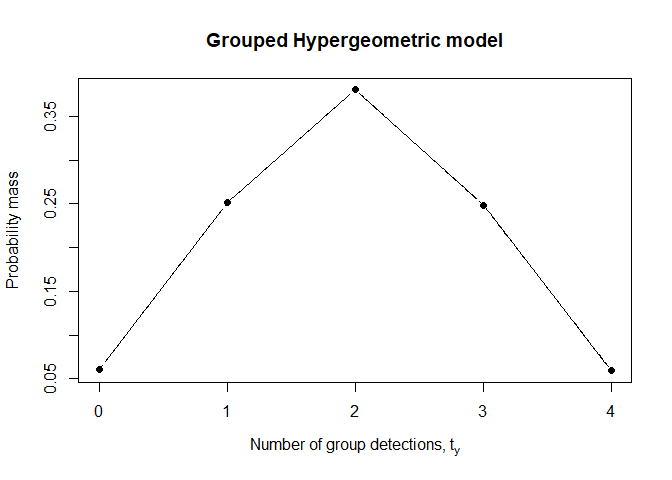
\includegraphics[width=1\linewidth]{man/figures/README-PMF HG Group-1}

In the similar way, the PMF can be calculated assuming item-level
imperfect test as below:

\begin{Shaded}
\begin{Highlighting}[]
\NormalTok{PRty.HG.item }\OtherTok{\textless{}{-}} \FunctionTok{sapply}\NormalTok{(ty.values, }\ControlFlowTok{function}\NormalTok{(ty) }\FunctionTok{pmfHG.imperfect.item}\NormalTok{(ty,}
    \AttributeTok{N =} \DecValTok{100}\NormalTok{, }\AttributeTok{barN =} \DecValTok{4}\NormalTok{, }\AttributeTok{Tx =} \DecValTok{20}\NormalTok{, }\AttributeTok{b =}\NormalTok{ b, }\AttributeTok{delta =} \FloatTok{0.7}\NormalTok{, }\AttributeTok{lambda =} \FloatTok{0.8}\NormalTok{,}
    \AttributeTok{verbose =} \ConstantTok{FALSE}\NormalTok{))}
\NormalTok{PRty.HG.item}
\CommentTok{\#\textgreater{} [1] 0.002993711 0.040346066 0.198811210 0.424987223 0.332861789}
\end{Highlighting}
\end{Shaded}

Expectation and variance of the grouped HG distribution for the number
of contaminated groups can be obtained as below:

\begin{Shaded}
\begin{Highlighting}[]
\NormalTok{ExpVarHG.imperfect.item }\OtherTok{\textless{}{-}} \FunctionTok{ExpVarHG.imperfect}\NormalTok{(}\AttributeTok{N =} \DecValTok{100}\NormalTok{, }\AttributeTok{Tx =} \DecValTok{20}\NormalTok{,}
    \AttributeTok{barN =} \DecValTok{4}\NormalTok{, }\AttributeTok{b =} \DecValTok{4}\NormalTok{, }\AttributeTok{delta =} \FloatTok{0.7}\NormalTok{, }\AttributeTok{lambda =} \FloatTok{0.8}\NormalTok{, }\AttributeTok{type =} \StringTok{"item"}\NormalTok{)}
\NormalTok{ExpVarHG.imperfect.item}\SpecialCharTok{$}\NormalTok{expectation}
\CommentTok{\#\textgreater{} [1] 3.044377}
\NormalTok{ExpVarHG.imperfect.item}\SpecialCharTok{$}\NormalTok{variance}
\CommentTok{\#\textgreater{} [1] 0.7180313}

\NormalTok{ExpVarHG.perfect.group }\OtherTok{\textless{}{-}} \FunctionTok{ExpVarHG.imperfect}\NormalTok{(}\AttributeTok{N =} \DecValTok{100}\NormalTok{, }\AttributeTok{Tx =} \DecValTok{20}\NormalTok{,}
    \AttributeTok{barN =} \DecValTok{4}\NormalTok{, }\AttributeTok{b =} \DecValTok{4}\NormalTok{, }\AttributeTok{delta =} \DecValTok{1}\NormalTok{, }\AttributeTok{lambda =} \DecValTok{1}\NormalTok{, }\AttributeTok{type =} \StringTok{"group"}\NormalTok{)}
\NormalTok{ExpVarHG.perfect.group}\SpecialCharTok{$}\NormalTok{expectation}
\CommentTok{\#\textgreater{} [1] 2.386647}
\NormalTok{ExpVarHG.perfect.group}\SpecialCharTok{$}\NormalTok{variance}
\CommentTok{\#\textgreater{} [1] 0.8797255}
\end{Highlighting}
\end{Shaded}

The Fisher Information for the number of contaminated items in the
population \(T_x\) can be calculated as below assuming group and item
level imperfect sensitivity and specificity:

\begin{Shaded}
\begin{Highlighting}[]
\NormalTok{Tx\_values }\OtherTok{\textless{}{-}} \FunctionTok{c}\NormalTok{(}\DecValTok{0}\SpecialCharTok{:}\DecValTok{80}\NormalTok{)}
\CommentTok{\# Different cases: Item level sensitivity}
\NormalTok{FI\_case1\_AD\_Based\_group }\OtherTok{\textless{}{-}} \FunctionTok{sapply}\NormalTok{(Tx\_values, }\ControlFlowTok{function}\NormalTok{(Tx) }\FunctionTok{FIpmfHG.Tx.imperfect}\NormalTok{(Tx,}
    \AttributeTok{N =} \DecValTok{100}\NormalTok{, }\AttributeTok{b =} \DecValTok{4}\NormalTok{, }\AttributeTok{barN =} \DecValTok{4}\NormalTok{, }\AttributeTok{delta =} \DecValTok{1}\NormalTok{, }\AttributeTok{lambda =} \DecValTok{1}\NormalTok{, }\AttributeTok{method =} \StringTok{"AD"}\NormalTok{,}
    \AttributeTok{type =} \StringTok{"group"}\NormalTok{, }\AttributeTok{verbose =} \ConstantTok{FALSE}\NormalTok{))}
\NormalTok{FI\_case1\_AD\_Based\_Item }\OtherTok{\textless{}{-}} \FunctionTok{sapply}\NormalTok{(Tx\_values, }\ControlFlowTok{function}\NormalTok{(Tx) }\FunctionTok{FIpmfHG.Tx.imperfect}\NormalTok{(Tx,}
    \AttributeTok{N =} \DecValTok{100}\NormalTok{, }\AttributeTok{b =} \DecValTok{4}\NormalTok{, }\AttributeTok{barN =} \DecValTok{4}\NormalTok{, }\AttributeTok{delta =} \DecValTok{1}\NormalTok{, }\AttributeTok{lambda =} \DecValTok{1}\NormalTok{, }\AttributeTok{method =} \StringTok{"AD"}\NormalTok{,}
    \AttributeTok{type =} \StringTok{"item"}\NormalTok{, }\AttributeTok{verbose =} \ConstantTok{FALSE}\NormalTok{))}
\FunctionTok{plot}\NormalTok{(Tx\_values, FI\_case1\_AD\_Based\_group, }\AttributeTok{type =} \StringTok{"l"}\NormalTok{, }\AttributeTok{col =} \StringTok{"black"}\NormalTok{,}
    \AttributeTok{xlab =} \FunctionTok{expression}\NormalTok{(}\FunctionTok{paste}\NormalTok{(}\StringTok{"Number of Contaminated Items, "}\NormalTok{,}
\NormalTok{        T[x])), }\AttributeTok{ylab =} \StringTok{"Fisher Information: Hypergeometric"}\NormalTok{,}
    \AttributeTok{main =} \StringTok{"FI under HG: Group and item level imperfect test"}\NormalTok{,}
    \AttributeTok{lty =} \DecValTok{2}\NormalTok{)}
\FunctionTok{lines}\NormalTok{(Tx\_values, FI\_case1\_AD\_Based\_Item, }\AttributeTok{type =} \StringTok{"l"}\NormalTok{, }\AttributeTok{lty =} \DecValTok{2}\NormalTok{,}
    \AttributeTok{col =} \StringTok{"blue"}\NormalTok{)}
\FunctionTok{legend}\NormalTok{(}\StringTok{"topright"}\NormalTok{, }\AttributeTok{legend =} \FunctionTok{c}\NormalTok{(}\StringTok{"Group"}\NormalTok{, }\StringTok{"Item"}\NormalTok{), }\AttributeTok{col =} \FunctionTok{c}\NormalTok{(}\StringTok{"black"}\NormalTok{,}
    \StringTok{"blue"}\NormalTok{), }\AttributeTok{lty =} \FunctionTok{c}\NormalTok{(}\DecValTok{1}\NormalTok{, }\DecValTok{2}\NormalTok{), }\AttributeTok{bty =} \StringTok{"n"}\NormalTok{)}
\end{Highlighting}
\end{Shaded}

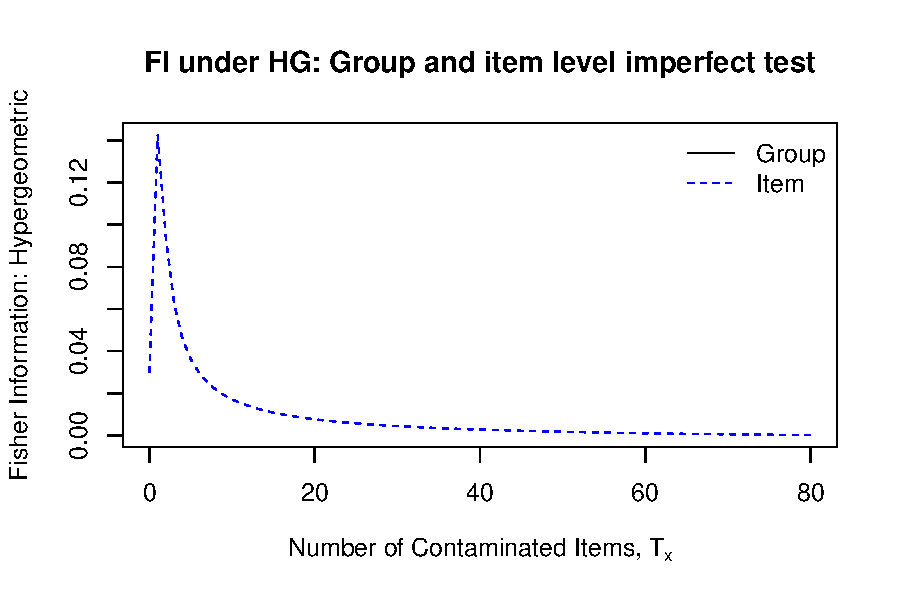
\includegraphics[width=1\linewidth]{man/figures/README-FI Item-1}

\subsection{Reference}\label{reference}

Sánchez-Moreno, P., Yánez, R. J., \& Dehesa, J. S. (2009, October).
Discrete densities and Fisher information. In Proceedings of the 14th
International Conference on Difference Equations and Applications.
Difference Equations and Applications. Istanbul, Turkey: Bahçesehir
University Press (pp.~291-298).

\end{document}
